\section{总体分析}

三个问题构成递进逻辑：问题1 建立物理模型（从光学原理到数学公式），问题2 在模型基础上设计算法并给出结果（从模型到数据），问题3 则识别模型假设的局限并升级模型（从近似到精确）。三个问题的模型并非各自独立，而是同一物理过程在不同精度层级上的展开。

\subsection{模型体系：一个模型、逐级升级}

核心物理场景为三层介质（空气/外延层/衬底）中的红外光干涉。问题1 建立了最简化的\textbf{双光束模型}（v1.0）：只计表面反射与衬底界面一次反射两束光的干涉，反射率谱为常数背景加单一余弦条纹，条纹频率与厚度成正比。问题2 基于 v1.0 模型，设计了三种从不同数据域独立反演厚度的算法（极值回归、谱域 FFT、全谱拟合），经逆方差融合与双重一致性检验后给出最终结果（v1.5）。问题3 将模型升级为\textbf{Airy 多光束模型}（v2.0）：考虑外延层内所有往返反射束的相干叠加，并显式引入衬底 Drude 介电函数的频变相位。三个版本的数学连续性已获数值验证：v2.0 在界面反射系数乘积 $q=|r_{10}r_{12}|\to 0$ 时精确退化为 v1.0/v1.5（偏差 $3.9\times 10^{-16}$，机器精度）。

\begin{figure}[H]
  \centering
  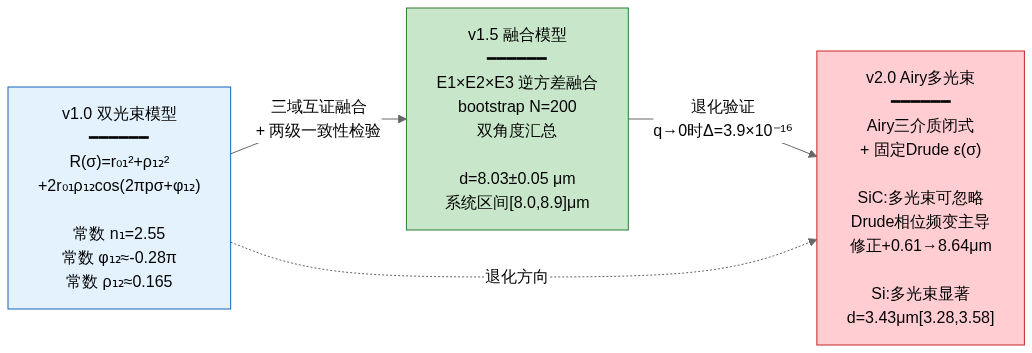
\includegraphics[width=0.95\textwidth]{../../03_结果与图表/最终图表/figM2_model_hierarchy.png}
  \caption{模型体系递进关系（v1.0 → v1.5 → v2.0）}
  \label{fig:model_hierarchy}
\end{figure}

\subsection{验证体系：四条独立验证线}

本文的可靠性论证不依赖单一指标，而是通过四条独立验证线构成完整体系：（1）合成数据闭环验证——以已知真值生成合成谱，全管线反演，检查恢复偏差；（2）双入射角互证——同一晶圆在 10\degree 和 15\degree 两份独立数据上分别反演，比对一致性；（3）残差诊断——分析拟合残差的结构与量级，判断模型是否穷尽数据中的物理信息；（4）多算法交叉——三种算法、两个角度共六个独立估计两两对照，逐一归因差异。四条验证线形成"算法自身无偏 $\to$ 数据间自洽 $\to$ 模型残差可控且归因 $\to$ 独立路径互证"的逻辑链。